% Anatomy of one explicit Runge-Kutta step, drawn for the classic RK4.
% Rows, top to bottom: the step's initial state, the stage states built by
% `combine`, the tendency evaluations, the tendency registers, and the single
% closing `accumulate` that produces the new state in place.
\documentclass[tikz,border=6pt]{standalone}
\usepackage{amsmath}
\usetikzlibrary{positioning,fit,arrows.meta,calc,backgrounds}

% Palette: states blue, tendencies orange, operations grey.
\definecolor{statecol}{RGB}{214,230,245}
\definecolor{tendcol}{RGB}{252,226,196}
\definecolor{opcol}{RGB}{235,235,235}
\definecolor{bandcol}{RGB}{247,247,247}

\begin{document}
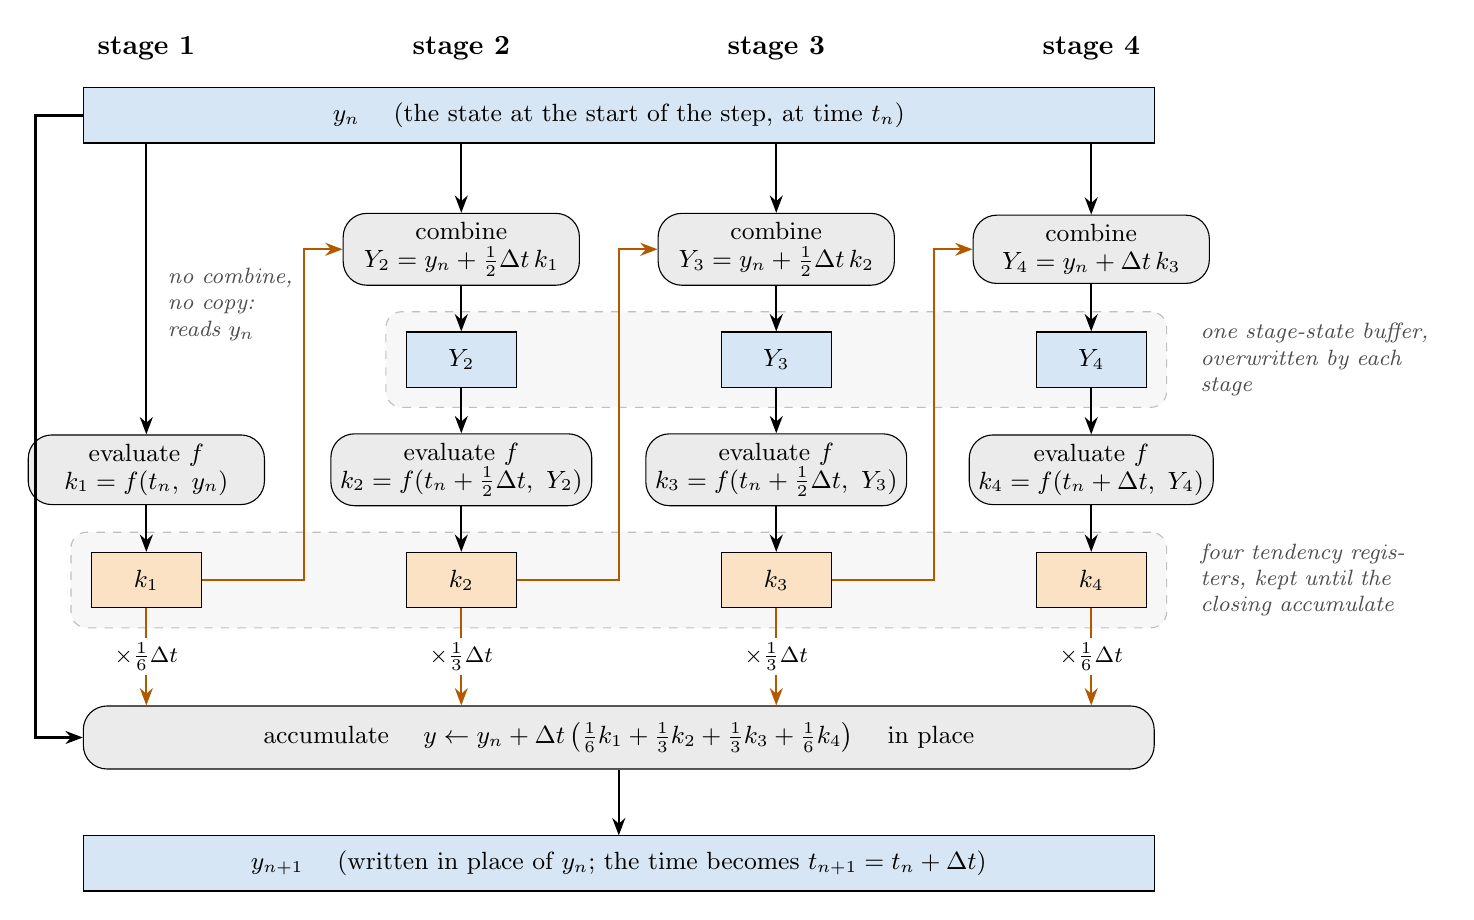
\begin{tikzpicture}[
    font=\small,
    >={Stealth[length=2.2mm]},
    state/.style={draw, fill=statecol, minimum height=7mm, minimum width=14mm},   % data: a model state
    tend/.style={draw, fill=tendcol, minimum height=7mm, minimum width=14mm},     % data: a tendency register
    op/.style={draw, rounded corners=3mm, fill=opcol, minimum height=8mm,
               minimum width=30mm, align=center},                                 % an operation on the data
    flow/.style={->, thick},                                                      % data flowing into an operation
    coef/.style={font=\footnotesize, fill=white, inner sep=1.5pt},                % coefficient label on an arrow
    note/.style={font=\footnotesize\itshape, align=left, text=black!70},          % explanatory side note
  ]

  % ---- grid: column of stage i at x = 4(i-1), one row per kind of object ----
  \def\yHead{0.85}    % row of the stage headers
  \def\yInit{0}      % row of the step's initial state y_n
  \def\yComb{-1.7}   % row of the combine operations
  \def\yStag{-3.1}   % row of the stage states Y_i
  \def\yEval{-4.5}   % row of the tendency evaluations
  \def\yTend{-5.9}   % row of the tendency registers k_i
  \def\yAccu{-7.9}   % row of the closing accumulate
  \def\yNext{-9.5}   % row of the new state y_{n+1}

  % ---- stage headers ----
  \foreach \i in {1,...,4} {
    \node[font=\bfseries] (h\i) at ({4*(\i-1)}, \yHead) {stage \i};               % header above each stage column
  }

  % ---- the step's initial state, read by every stage ----
  \node[state, minimum width=136mm] (yn) at (6, \yInit)
       {$y_n$ \quad (the state at the start of the step, at time $t_n$)};          % one wide box spanning all columns

  % ---- stage 1: evaluated on y_n itself ----
  \node[op] (f1) at (0, \yEval) {evaluate $f$\\[-1pt]$k_1 = f(t_n,\ y_n)$};       % first tendency, straight from y_n
  \draw[flow] (yn.south -| f1) -- (f1.north);                                      % y_n read directly, skipping combine
  \node[note, anchor=west, text width=17mm] at (0.15, {(\yComb+\yStag)/2})
       {no combine, no copy: reads $y_n$};                                         % why stage 1 has no stage state

  % ---- stages 2-4: combine, then evaluate on the stage state ----
  % \i = stage, \a = its coefficient a_{i,i-1} (as text), \c = its time offset c_i (as text)
  \foreach \i/\a/\c in {2/{\tfrac12\Delta t}/{\tfrac12\Delta t},
                        3/{\tfrac12\Delta t}/{\tfrac12\Delta t},
                        4/{\Delta t}/{\Delta t}} {
    \pgfmathtruncatemacro{\x}{4*(\i-1)}                                            % x position of this column
    \node[op] (c\i) at (\x, \yComb)
         {combine\\[-1pt]$Y_\i = y_n + \a\, k_{\the\numexpr\i-1\relax}$};          % stage state from y_n and k_{i-1}
    \node[state] (Y\i) at (\x, \yStag) {$Y_\i$};                                   % the stage state it produces
    \node[op] (f\i) at (\x, \yEval)
         {evaluate $f$\\[-1pt]$k_\i = f(t_n + \c,\ Y_\i)$};                         % tendency at the stage time
    \draw[flow] (yn.south -| c\i) -- (c\i.north);                                  % y_n feeds the combine
    \draw[flow] (c\i) -- (Y\i);                                                    % combine writes Y_i
    \draw[flow] (Y\i) -- (f\i);                                                    % Y_i feeds the evaluation
  }

  % ---- tendency registers, one per stage ----
  \foreach \i in {1,...,4} {
    \node[tend] (k\i) at ({4*(\i-1)}, \yTend) {$k_\i$};                            % register holding k_i
    \draw[flow] (f\i) -- (k\i);                                                    % evaluation writes k_i
  }

  % ---- k_{i-1} feeds the combine of stage i, routed through the gap between columns ----
  % (its coefficient is written in the combine box it enters)
  \foreach \j/\i in {1/2, 2/3, 3/4} {
    \pgfmathsetmacro{\gx}{4*(\j-1)+2}                                              % x of the gap right of column j
    \draw[flow, draw=orange!70!black]
         (k\j.east) -- (\gx, \yTend) -- (\gx, \yComb) -- (c\i.west);               % right, up the gap, into combine
  }

  % ---- background bands naming the shared buffers ----
  \begin{scope}[on background layer]
    \node[fill=bandcol, draw=black!25, dashed, rounded corners=2mm, inner sep=2.5mm,
          fit=(Y2)(Y4)] (stageband) {};                                            % band behind Y_2..Y_4
    \node[fill=bandcol, draw=black!25, dashed, rounded corners=2mm, inner sep=2.5mm,
          fit=(k1)(k4)] (tendband) {};                                             % band behind k_1..k_4
  \end{scope}
  \node[note, anchor=west, text width=30mm] at ($(stageband.east)+(0.3,0)$)
       {one stage-state buffer, overwritten by each stage};                         % Y_2..Y_4 share storage
  \node[note, anchor=west, text width=30mm] at ($(tendband.east)+(0.3,0)$)
       {four tendency registers, kept until the closing accumulate};               % why rk4 keeps 4 registers

  % ---- the closing accumulate ----
  \node[op, minimum width=136mm] (acc) at (6, \yAccu)
       {accumulate \quad $y \leftarrow y_n + \Delta t\,\bigl(\tfrac16 k_1 + \tfrac13 k_2
        + \tfrac13 k_3 + \tfrac16 k_4\bigr)$ \quad in place};                      % the closing update
  \foreach \i/\b in {1/{\tfrac16},2/{\tfrac13},3/{\tfrac13},4/{\tfrac16}} {
    \draw[flow, draw=orange!70!black] (k\i.south) -- (k\i.south |- acc.north)
         node[coef, midway] {$\times\b\Delta t$};                                   % each k_i with its weight b_i dt
  }
  \draw[flow] (yn.west) -- ++(-0.6,0) |- (acc.west);                               % y_n itself enters the final update

  % ---- the new state, written in place of y_n ----
  \node[state, minimum width=136mm] (ynext) at (6, \yNext)
       {$y_{n+1}$ \quad (written in place of $y_n$; the time becomes $t_{n+1} = t_n + \Delta t$)}; % result of the step
  \draw[flow] (acc) -- (ynext);                                                    % accumulate produces y_{n+1}

\end{tikzpicture}
\end{document}
